\subsubsection{Projektplanung und technische Einschätzung}

Sprint 1 fokussierte auf die technische Machbarkeitsanalyse und strategische Projektausrichtung in enger Abstimmung mit Fachexperten und Stakeholdern.

\textbf{Technische Beratung (17.01.2025):}
Ein Lehrbeauftragter des Moduls \textit{Digital Art} (Hochschule Reutlingen) empfahl die Integration von MediaPipe als Subprozess für das Live-RGB-Signal der Kinect. Ziel: Skeleton-Generierung für bewegungsbasierte Trigger-Ableitung.

Ich erstellte eine TELOS-Analyse (siehe Appendix) um die Machbarkeit des Projektes einzuschätzen, was einen guten Überblick über bestehende Technologien geschafft hat.

\textbf{Technologie-Evaluation:}
Parallel zur MediaPipe-Integration wurde das native Kinect-Skeleton-Tracking evaluiert, was die Entwicklung eines hybriden Dual-Source-Ansatzes ermöglichte.

\subsubsection{Stakeholder-Entscheidungen}

Das Stakeholder-Meeting Ende Januar definierte die Kernarchitektur des M.A.S.K.-Systems:

\textbf{Hybrid-Tracking-Konzept:}
\begin{itemize}
    \item \textbf{Dual-Source-Input:} MediaPipe und Kinect als alternative/komplementäre Datenquellen
    \item \textbf{Datenfusion:} Skeleton-Synchronisation mit Kalman-Filter-Glättung
    \item \textbf{Trigger-Pipeline:} Bewegungsanalyse basierend auf fusionierten Skeleton-Daten
    \item \textbf{Adaptive Optimierung:} MediaPipe als Fallback bei Kinect-Limitationen
\end{itemize}

\textbf{Bewegungsanalyseparameter:}
Geschwindigkeit, Beschleunigung, Rotation und Winkelbeziehungen zwischen Skeleton-Nodes.

\begin{figure}[H]
    \centering
    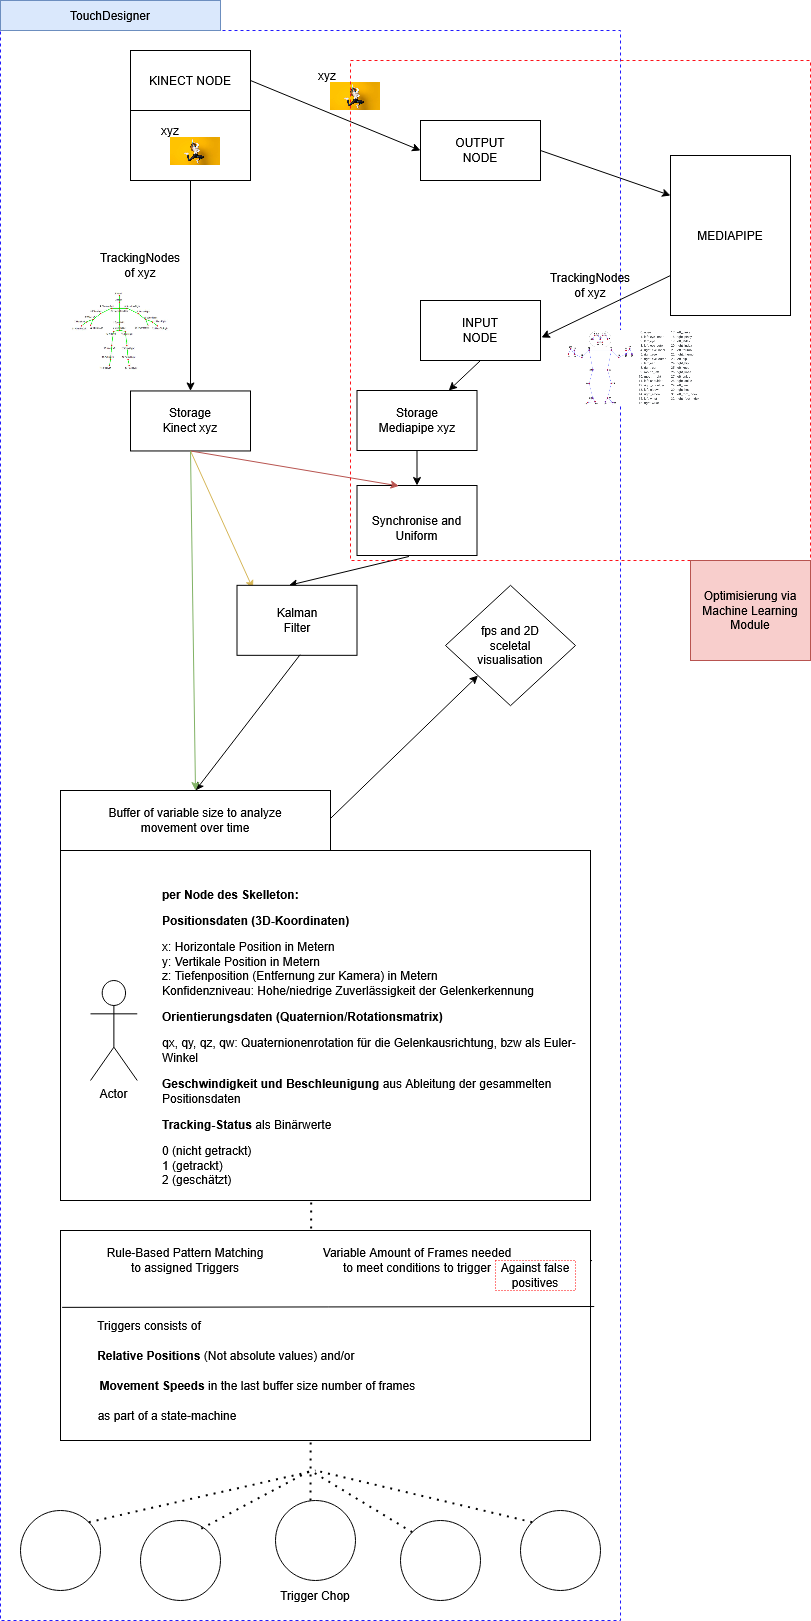
\includegraphics[width=0.7\textwidth]{images/MASK.png}
    \caption{M.A.S.K. Systemarchitektur: Analyse- und Triggerprozess}
    \label{fig:mask_architecture}
\end{figure}

\subsubsection{Algorithmusdesign}

\begin{algorithm}[H]
\caption{Hauptverarbeitungsschleife (Frame-synchronisiert)}\label{alg:main_processing}
\begin{algorithmic}[1]
    \State $\text{processedSkeleton}[] \leftarrow \text{buffer}$
    \State \textbf{log}("Frame processing initiated")
    \State $\text{kinect\_data} \leftarrow \text{receiveKinectSkeleton()}$
    \State $\text{mediapipe\_data} \leftarrow \text{processRGBStream()}$
    \If{$\text{mediapipe\_data} \neq \text{null}$}
        \State \textbf{log}("MediaPipe data available, performing fusion")
        \State $\text{skeleton} \leftarrow \text{fusionProcess}(\text{kinect\_data}, \text{mediapipe\_data})$
    \Else
        \State \textbf{log}("MediaPipe unavailable, Kinect-only mode")
        \State $\text{skeleton} \leftarrow \text{kinect\_data}$
    \EndIf
    \State $\text{skeleton} \leftarrow \text{applyKalmanFilter}(\text{skeleton})$
    \State $\text{processedSkeleton} \leftarrow \text{analyzeMovement}(\text{skeleton}, \text{buffer})$
    \State $\text{buffer.append}(\text{processedSkeleton})$
    \State \textbf{evaluateTriggers}(\text{buffer})
\end{algorithmic}
\end{algorithm}

\subsubsection{Choreographie-Meeting (10.03.2025)}

\textbf{Teilnehmer:} Projektteam Filmakademie Ludwigsburg, M.A.S.K.-Entwicklungsteam

\textbf{Definierte Tracking-Szenarien:}

\begin{enumerate}
    \item \textbf{Segment 1 - Aktivierungssequenz:}
    \begin{itemize}
        \item Skeleton-Detection löst Beamer-Visual-Aktivierung aus
        \item Fokus: Hand- und Arm-Tracking
        \item Sequenzielle Trigger-Kaskade implementieren
    \end{itemize}
    
    \item \textbf{Segment 2 - Top-Down-Perspektive:}
    \begin{itemize}
        \item Kalibrierung: Beamer-Kinect-Visual-Relation
        \item Overhead-Tracking für Bodenprojektionen
    \end{itemize}
    
    \item \textbf{Segment 3 - Bewegungsresponsive Visuals:}
    \begin{itemize}
        \item Spezifische Gesten-zu-Visual-Mappings
        \item Real-time Bewegungserkennung
    \end{itemize}
    
    \item \textbf{Segment 4 - Erweiterte Funktionen:}
    \begin{itemize}
        \item Kopf- und Arm-Bewegungstrigger
        \item Tiefensensor-basierte Performer-Segmentierung
    \end{itemize}
\end{enumerate}

\textbf{Sprint 2 Deliverables:}
\begin{itemize}
    \item TouchDesigner-Testumgebung (\texttt{.toe}-Datei)
    \item Mobile Kinect-Tracking-Validierung
    \item Multi-Person-Filtering (Kameramann-Ausblendung)
\end{itemize}